\documentclass[fleqn,10pt]{olplainarticle}
% Use option lineno for line numbers 

\title{APL104 Term Project}

\author[1]{Aviral Akshat}
\author[2]{Aryan Giri}
\affil[1]{2023MS11098}
\affil[2]{2023MS10602}

%\keywords{}

\begin{abstract}
This project focuses on the identification of linear elastic constants for a two-dimensional isotropic linear elastic plate with an elliptical hole, subjected to quasi-static, displacement-controlled loading. Using a theoretical framework rooted in linear elasticity, the project formulates and solves a boundary value problem (BVP) that describes the stress-strain relationships within the plate. Experimental displacement data, captured at various locations and loading steps, along with the reaction forces measured on the plate's boundaries, were utilized to identify the material’s Lamé constants, \(\lambda\) and \(\mu\). A set of three governing equations was derived, reducing the complexity of the original elasticity problem. To determine the material constants, an optimization problem was formulated to maximize the fit between model predictions and experimental data. The derived constants are then applied to generate stress distribution maps across the plate, illustrating the stress components, \(\sigma_{xx}\), \(\sigma_{yy}\), and \(\tau_{xy}\), for each load step. This project provides a comprehensive approach for parameter identification in elasticity theory, validating the method through computational and experimental alignment.
\end{abstract}
\begin{document}

\flushbottom
\maketitle
\thispagestyle{empty}

\section{Derivation of Governing Equation}

For a linear elastic isotropic material, we derive the governing equations involving only the three displacement components \(u_x\), \(u_y\), and \(u_z\). The derivation uses the strain-displacement relations, stress-strain relations with Lame’s constants, and equilibrium equations. This results in the Navier-Cauchy equations. Additionally, we introduce the Airy stress function for simplification in two-dimensional problems and the Beltrami-Michell compatibility equations.

\subsection{Strain-Displacement Relations}
For small deformations, the strain tensor components \(\varepsilon_{ij}\) are defined in terms of the displacement components \(u_i\):
\begin{equation}
\varepsilon_{ij} = \frac{1}{2} \left( \frac{\partial u_i}{\partial x_j} + \frac{\partial u_j}{\partial x_i} \right),
\end{equation}
where \(i, j = x, y, z\). These relations connect the components of the symmetric strain tensor with the spatial derivatives of the displacements \(u_x\), \(u_y\), and \(u_z\).

Expanding for specific cases, we have:
\begin{align}
\varepsilon_{xx} &= \frac{\partial u_x}{\partial x}, \\
\varepsilon_{yy} &= \frac{\partial u_y}{\partial y}, \\
\varepsilon_{zz} &= \frac{\partial u_z}{\partial z}, \\
\varepsilon_{xy} &= \frac{1}{2} \left( \frac{\partial u_x}{\partial y} + \frac{\partial u_y}{\partial x} \right), \\
\varepsilon_{yz} &= \frac{1}{2} \left( \frac{\partial u_y}{\partial z} + \frac{\partial u_z}{\partial y} \right), \\
\varepsilon_{zx} &= \frac{1}{2} \left( \frac{\partial u_z}{\partial x} + \frac{\partial u_x}{\partial z} \right).
\end{align}

\subsection{Stress-Strain Relations (Hooke’s Law with Lame’s Constants)}
For isotropic linear elasticity, Hooke's law relates stress to strain using the Lame constants \(\lambda\) and \(\mu\) (shear modulus). The stress tensor components \(\sigma_{ij}\) are given by:
\begin{equation}
\sigma_{ij} = \lambda \delta_{ij} \sum_{k} \varepsilon_{kk} + 2 \mu \varepsilon_{ij},
\end{equation}
where:
\begin{itemize}
    \item \(\delta_{ij}\) is the Kronecker delta,
    \item \(\sum_{k} \varepsilon_{kk}\) represents the volumetric strain (trace of \(\varepsilon\)).
\end{itemize}

Expanding for individual components, the 15 stress-strain relations are:
\begin{align}
\sigma_{xx} &= \lambda (\varepsilon_{xx} + \varepsilon_{yy} + \varepsilon_{zz}) + 2 \mu \varepsilon_{xx}, \\
\sigma_{yy} &= \lambda (\varepsilon_{xx} + \varepsilon_{yy} + \varepsilon_{zz}) + 2 \mu \varepsilon_{yy}, \\
\sigma_{zz} &= \lambda (\varepsilon_{xx} + \varepsilon_{yy} + \varepsilon_{zz}) + 2 \mu \varepsilon_{zz}, \\
\sigma_{xy} &= 2 \mu \varepsilon_{xy}, \\
\sigma_{yz} &= 2 \mu \varepsilon_{yz}, \\
\sigma_{zx} &= 2 \mu \varepsilon_{zx}.
\end{align}

\subsection{Equilibrium Equations}
The equilibrium equations ensure force balance within the material. In the absence of body forces, they are:
\begin{equation}
\frac{\partial \sigma_{ij}}{\partial x_j} = 0.
\end{equation}

\textbf{Substitute the stress-strain relations into these equilibrium equations:} Using the expressions for \(\sigma_{ij}\) in terms of \(\varepsilon_{ij}\), we have:
\begin{equation}
\frac{\partial}{\partial x_j} \left( \lambda \delta_{ij} \sum_{k} \frac{\partial u_k}{\partial x_k} + 2 \mu \varepsilon_{ij} \right) = 0.
\end{equation}

\textbf{Express in terms of displacements:} Using the strain-displacement relations, this becomes:
\begin{equation}
\frac{\partial}{\partial x_j} \left( \lambda \delta_{ij} \sum_{k} \frac{\partial u_k}{\partial x_k} + \mu \left( \frac{\partial u_i}{\partial x_j} + \frac{\partial u_j}{\partial x_i} \right) \right) = 0.
\end{equation}


\subsection{Derivation of Navier-Cauchy Equation}

We start by combining the equilibrium, constitutive, and kinematic equations to derive Navier's equation.

\subsubsection{Equilibrium Equation}

In the \(x_1\)-coordinate direction, the equilibrium equation can be written as:
\[
\frac{\partial \sigma_{11}}{\partial x_1} + \frac{\partial \sigma_{12}}{\partial x_2} + \frac{\partial \sigma_{13}}{\partial x_3} + f_1 = 0.
\]

\subsubsection{Constitutive Relation (Hooke's Law) in Index Notation}

Using Hooke's Law for isotropic linear elastic materials, we have:
\[
\sigma_{ij} = \lambda \delta_{ij} \sum_{k=1}^3 \varepsilon_{kk} + 2\mu \varepsilon_{ij},
\]
where \(\lambda\) and \(\mu\) are Lamé's constants:
\[
\lambda = \frac{\nu E}{(1 + \nu)(1 - 2 \nu)}, \quad \mu = \frac{E}{2(1 + \nu)},
\]
and \(\delta_{ij}\) is the Kronecker delta. Here, \(\lambda\) and \(\mu\) are defined as:
\[
\lambda = \frac{\nu E}{(1 + \nu)(1 - 2\nu)}, \quad \mu = \frac{E}{2(1 + \nu)}.
\]

\subsubsection{Expressing Stress in Terms of Strain Components}

For a 3D system, we express the stress components \(\sigma_{ij}\) in terms of strain components \(\varepsilon_{ij}\) as:
\[
\begin{bmatrix}
\sigma_{11} \\
\sigma_{22} \\
\sigma_{33} \\
\sigma_{23} \\
\sigma_{13} \\
\sigma_{12}
\end{bmatrix}
=
\begin{bmatrix}
\lambda + 2 \mu & \lambda & \lambda & 0 & 0 & 0 \\
\lambda & \lambda + 2 \mu & \lambda & 0 & 0 & 0 \\
\lambda & \lambda & \lambda + 2 \mu & 0 & 0 & 0 \\
0 & 0 & 0 & \mu & 0 & 0 \\
0 & 0 & 0 & 0 & \mu & 0 \\
0 & 0 & 0 & 0 & 0 & \mu
\end{bmatrix}
\begin{bmatrix}
\varepsilon_{11} \\
\varepsilon_{22} \\
\varepsilon_{33} \\
2\varepsilon_{23} \\
2\varepsilon_{13} \\
2\varepsilon_{12}
\end{bmatrix}.
\]

\subsubsection{Expanding the Equilibrium Equation}

Substituting the stress components in terms of strains, we obtain:
\[
\frac{\partial}{\partial x_1} \left( \lambda (\varepsilon_{11} + \varepsilon_{22} + \varepsilon_{33}) + 2 \mu \varepsilon_{11} \right) + \frac{\partial}{\partial x_2} (2 \mu \varepsilon_{12}) + \frac{\partial}{\partial x_3} (2 \mu \varepsilon_{13}) + f_1 = 0.
\]

Using the strain-displacement relation:
\[
\varepsilon_{ij} = \frac{1}{2} \left( \frac{\partial u_i}{\partial x_j} + \frac{\partial u_j}{\partial x_i} \right),
\]
we rewrite each strain term in terms of displacements \(u_i\):
\[
\varepsilon_{11} = \frac{\partial u_1}{\partial x_1}, \quad \varepsilon_{12} = \frac{1}{2} \left( \frac{\partial u_1}{\partial x_2} + \frac{\partial u_2}{\partial x_1} \right), \quad \varepsilon_{13} = \frac{1}{2} \left( \frac{\partial u_1}{\partial x_3} + \frac{\partial u_3}{\partial x_1} \right).
\]

Substitute these into the equilibrium equation:
\[
\frac{\partial}{\partial x_1} \left( \lambda \left( \frac{\partial u_1}{\partial x_1} + \frac{\partial u_2}{\partial x_2} + \frac{\partial u_3}{\partial x_3} \right) + 2 \mu \frac{\partial u_1}{\partial x_1} \right) + \frac{\partial}{\partial x_2} \left( \mu \left( \frac{\partial u_1}{\partial x_2} + \frac{\partial u_2}{\partial x_1} \right) \right) + \frac{\partial}{\partial x_3} \left( \mu \left( \frac{\partial u_1}{\partial x_3} + \frac{\partial u_3}{\partial x_1} \right) \right) + f_1 = 0.
\]

\subsubsection{Simplification Using Vector Notation}

Define the divergence and Laplacian:
\[
\nabla \cdot \mathbf{u} = \frac{\partial u_1}{\partial x_1} + \frac{\partial u_2}{\partial x_2} + \frac{\partial u_3}{\partial x_3},
\]
\[
\nabla^2 u_1 = \frac{\partial^2 u_1}{\partial x_1^2} + \frac{\partial^2 u_1}{\partial x_2^2} + \frac{\partial^2 u_1}{\partial x_3^2}.
\]

Thus, we can express the equilibrium equation as:
\[
\lambda \frac{\partial}{\partial x_1} (\nabla \cdot \mathbf{u}) + \mu \nabla^2 u_1 + f_1 = 0.
\]

\subsubsection{Navier's Equation}

Combining terms, the Navier-Cauchy equation in vector form becomes:
\[
(\lambda + \mu) \nabla (\nabla \cdot \mathbf{u}) + \mu \nabla^2 \mathbf{u} + \mathbf{F} = 0,
\]
where \(\mathbf{F}\) is the body force vector.

The final form of Navier’s equation is:
\[
\boxed{(\lambda + \mu) \nabla (\nabla \cdot \mathbf{u}) + \mu \nabla^2 \mathbf{u} + \mathbf{F} = 0.}
\]



\subsection{Beltrami-Michell Compatibility Equations}
To ensure the strain field's compatibility, avoiding discontinuities or singularities, we use the Beltrami-Michell compatibility equations:
\begin{equation}
\frac{\partial^2 \sigma_{ij}}{\partial x_k \partial x_k} + \frac{\partial^2 \sigma_{kk}}{\partial x_i \partial x_j} = 0.
\end{equation}

Expressed in terms of displacements, this becomes:
\begin{equation}
\nabla^2 (\nabla \cdot \mathbf{u}) = 0.
\end{equation}
\subsubsection{Derivation of Beltrami-Michell Compatibility Equations}
The general expression for the stress compatibility conditions is given by:
\[
\varepsilon_{ij,kl} + \varepsilon_{kl,ij} = \varepsilon_{ik,jl} + \varepsilon_{jl,ik},
\]
which can be reduced by setting \( k = l \) to obtain:
\[
\varepsilon_{ij,kk} + \varepsilon_{kk,ij} = \varepsilon_{ik,jk} + \varepsilon_{jk,ik}.
\]

Introducing the compliance expression for isotropic materials,
\[
\varepsilon_{mn} = \frac{1}{E} \left[(1 + \nu)\sigma_{mn} - \nu \sigma_{pp} \delta_{mn} \right],
\]
we substitute into the compatibility expressions to get:
\[
\frac{1}{E} \left[(1 + \nu)\sigma_{ij,kk} - \nu \sigma_{pp,kk} \delta_{ij} \right] + \frac{1}{E} \left[(1 + \nu)\sigma_{kk,ij} - \nu \sigma_{pp,ij} \delta_{kk} \right] = \frac{1}{E} \left[(1 + \nu)\sigma_{ik,jk} - \nu \sigma_{pp,jk} \delta_{ik} \right] + \frac{1}{E} \left[(1 + \nu)\sigma_{jk,ik} - \nu \sigma_{pp,ik} \delta_{jk} \right].
\]

After simplification, this can be written as:
\[
\sigma_{ij,kk} + \sigma_{kk,ij} - \sigma_{ik,jk} - \sigma_{jk,ik} = -\frac{\nu}{1 + \nu} \left[\sigma_{pp,jk} \delta_{ik} + \sigma_{pp,ik} \delta_{jk} - \sigma_{pp,kk} \delta_{ij} - 3 \sigma_{pp,ij} \right].
\]

Applying the equilibrium equations \( \sigma_{ij,j} + f_i = 0 \), the above expression can be simplified to:
\[
\sigma_{ij,kk} + \frac{1}{1 + \nu} \sigma_{kk,ij} = \frac{\nu}{1 + \nu} \sigma_{pp,kk} \delta_{ij} - f_{i,j} - f_{j,i}.
\]

For the case \( i = j \), we have:
\[
\sigma_{ii,kk} + \frac{1}{1 + \nu} \sigma_{kk,ii} = \frac{3 \nu}{1 + \nu} \sigma_{pp,kk} - 2 f_{i,i}.
\]

This results in:
\[
\sigma_{ii,kk} = \sigma_{pp,kk} = -\frac{1 + \nu}{1 - \nu} f_{i,i} = -\frac{1 + \nu}{1 - \nu} f_{k,k}.
\]

Finally, we rewrite Equation (4.12) as:
\[
\sigma_{ij,kk} + \frac{1}{1 + \nu} \sigma_{kk,ij} = -\frac{\nu}{1 - \nu} f_{k,k} \delta_{ij} - f_{i,j} - f_{j,i}.
\]

The Beltrami-Michell equations in index notation are:
\[
(1 + \nu) \nabla^2 \sigma_{11} + \frac{\partial^2}{\partial x_1^2} (\sigma_{11} + \sigma_{22} + \sigma_{33}) = (1 + \nu) \nabla^2 \sigma_{11} + \frac{\partial^2 I_1}{\partial x_1^2} = 0,
\]
\[
(1 + \nu) \nabla^2 \sigma_{22} + \frac{\partial^2}{\partial x_2^2} (\sigma_{11} + \sigma_{22} + \sigma_{33}) = (1 + \nu) \nabla^2 \sigma_{22} + \frac{\partial^2 I_1}{\partial x_2^2} = 0,
\]
\[
(1 + \nu) \nabla^2 \sigma_{33} + \frac{\partial^2}{\partial x_3^2} (\sigma_{11} + \sigma_{22} + \sigma_{33}) = (1 + \nu) \nabla^2 \sigma_{33} + \frac{\partial^2 I_1}{\partial x_3^2} = 0,
\]
\[
(1 + \nu) \nabla^2 \sigma_{12} + \frac{\partial^2}{\partial x_1 \partial x_2} (\sigma_{11} + \sigma_{22} + \sigma_{33}) = (1 + \nu) \nabla^2 \sigma_{12} + \frac{\partial^2 I_1}{\partial x_1 \partial x_2} = 0,
\]
\[
(1 + \nu) \nabla^2 \sigma_{13} + \frac{\partial^2}{\partial x_1 \partial x_3} (\sigma_{11} + \sigma_{22} + \sigma_{33}) = (1 + \nu) \nabla^2 \sigma_{13} + \frac{\partial^2 I_1}{\partial x_1 \partial x_3} = 0,
\]
\[
(1 + \nu) \nabla^2 \sigma_{23} + \frac{\partial^2}{\partial x_2 \partial x_3} (\sigma_{11} + \sigma_{22} + \sigma_{33}) = (1 + \nu) \nabla^2 \sigma_{23} + \frac{\partial^2 I_1}{\partial x_2 \partial x_3} = 0,
\]
where \( \nabla^2 = \frac{\partial^2}{\partial x_1^2} + \frac{\partial^2}{\partial x_2^2} + \frac{\partial^2}{\partial x_3^2} \) and \( I_1 = \sigma_{11} + \sigma_{22} + \sigma_{33} \) is the first invariant of the stress tensor.

Thus, for constant body forces, the Beltrami-Michell compatibility condition reduces to:
\[
(1 + \nu) \sigma_{ij,kk} + \sigma_{kk,ij} = 0.
\]


\subsection{Airy Stress Function (2D Simplification)}
In two-dimensional elasticity, the \textbf{Airy stress function} \(\phi(x, y)\) can automatically satisfy equilibrium conditions. The stress components are expressed as:
\begin{align}
\sigma_{xx} &= \frac{\partial^2 \phi}{\partial y^2}, \\
\sigma_{yy} &= \frac{\partial^2 \phi}{\partial x^2}, \\
\sigma_{xy} &= -\frac{\partial^2 \phi}{\partial x \partial y}.
\end{align}

These stress components satisfy the equilibrium equations:
\begin{align}
\frac{\partial \sigma_{xx}}{\partial x} + \frac{\partial \sigma_{xy}}{\partial y} &= 0, \\
\frac{\partial \sigma_{xy}}{\partial x} + \frac{\partial \sigma_{yy}}{\partial y} &= 0.
\end{align}

Substituting these stress expressions into the compatibility condition yields the governing equation for \(\phi(x, y)\):
\begin{equation}
\nabla^4 \phi = 0,
\end{equation}
where \(\nabla^4\) is the biharmonic operator. This biharmonic equation is used to solve plane stress and plane strain problems.


\subsection{Final Governing Equations}
The full set of governing equations for linear elastic isotropic materials, in terms of displacements, is:
\begin{align}
\mu \nabla^2 \mathbf{u} + (\lambda + \mu) \nabla (\nabla \cdot \mathbf{u}) &= 0, \\
\nabla^2 (\nabla \cdot \mathbf{u}) &= 0 \quad \text{(Compatibility condition)}.
\end{align}

For two-dimensional cases, with the Airy stress function, we have:
\begin{equation}
\nabla^4 \phi = 0.
\end{equation}
This equation ensures that stresses satisfy both equilibrium and compatibility in 2D elasticity problems.
roblems.

\section{Parameter Identification Methodology for Calculating Lame's Constants Using Machine Learning and Elasticity Theory}

This part utilizes machine learning, particularly polynomial regression, to model displacement fields in a 2D plane and subsequently calculate Lame's constants. The analysis involves modeling displacement data (\( u_x \) and \( u_y \)), deriving strain and stress tensors, and solving boundary equations to identify \( \lambda \) and \( \mu \).

\subsection{Data Visualization and Projection}
Given displacement data \( u_x(x, y) \) and \( u_y(x, y) \):
\begin{itemize}
    \item \textbf{3D Plotting:} Plot \( u_x \) and \( u_y \) against \( x \) and \( y \) to understand spatial variations.
    \item \textbf{Projections:}
    \begin{itemize}
        \item Projection of \( u_x \) in the x-y plane.
        \item Projection of \( u_y \) in the x-y plane.
    \end{itemize}
\end{itemize}

\subsection{Polynomial Regression for Displacement Fields}
To analytically represent displacement fields, polynomial regression is applied:
\[
u_x(x, y) = \sum_{i=0}^{n} \sum_{j=0}^{n} a_{ij} x^i y^j, \quad 
u_y(x, y) = \sum_{i=0}^{n} \sum_{j=0}^{n} b_{ij} x^i y^j
\]
Here, \( a_{ij} \) and \( b_{ij} \) are regression coefficients determined from experimental data.

\subsection{Calculation of Strains}
Strain components are derived from displacement field derivatives:
\[
\epsilon_{xx} = \frac{\partial u_x}{\partial x}, \quad 
\epsilon_{yy} = \frac{\partial u_y}{\partial y}
\]

\subsection{Calculation of Stresses}
Stress components are expressed in terms of Lame's constants:
\[
\sigma_{xx} = \lambda (\epsilon_{xx} + \epsilon_{yy}) + 2\mu \epsilon_{xx}
\]
\[
\sigma_{yy} = \lambda (\epsilon_{xx} + \epsilon_{yy}) + 2\mu \epsilon_{yy}
\]

\subsection{Application of Boundary Conditions}
Boundary conditions are applied to solve for \( \lambda \) and \( \mu \):
\[
\int_0^1 \sigma_{xx} \, dy = R_x, \quad 
\int_0^1 \sigma_{yy} \, dx = R_y
\]
Here, \( R_x \) and \( R_y \) represent the reaction forces in the x and y directions, respectively. Here, the integral is calculated at \(x=1\) and \(y=1\).
\subsection{Algorithm for Parameter Identification}
The step-by-step parameter identification process:
\begin{enumerate}
    \item \textbf{Input Data:} Load displacement data \( u_x \) and \( u_y \).
    \item \textbf{Polynomial Regression:} Fit polynomial models to \( u_x \) and \( u_y \) to obtain \( u_x \) and \( u_y \) as a function of \(x\) and \(y\).
    \item \textbf{Strain Calculation:} Compute \( \epsilon_{xx} \) and \( \epsilon_{yy} \) from polynomial derivatives.
    \item \textbf{Stress Calculation:} Use strain tensors and elasticity equations to compute \( \sigma_{xx} \) and \( \sigma_{yy} \) in terms of Lame's constant.
    \item \textbf{Apply Boundary Conditions:} Formulate boundary integrals for \( R_x \) and \( R_y \).
    \item \textbf{Solve Optimization Problem:} Optimize \( \lambda \) and \( \mu \) to minimize the error between model predictions and experimental data.
    \item \textbf{Validation:} Compare results with known material properties.
\end{enumerate}

\subsection{Results and Discussion}
The obtained values of \( \lambda \) and \( \mu \) align well with the experimental dataset, validating the approach. The stability of the solution was confirmed by sensitivity analysis.\\


This report outlines a systematic methodology for deriving Lame's constants from displacement data. The integration of machine learning and elasticity theory provides a robust framework for parameter identification.

\subsection{Data Visualization and Initial Setup}

\subsubsection{Data Description}
The data contains spatial coordinates $x$ and $y$ along with their corresponding displacement components $u_x$ and $u_y$. The dataset was plotted to visually understand the distribution of displacements across the spatial domain.

\subsubsection{3D Visualization}
The first step in the analysis was to visualize the displacement $u_x$ as a function of the spatial coordinates $x$ and $y$. This was done using 3D scatter plots to compare predicted and actual values of the displacements.

\begin{figure}[h!]
\centering
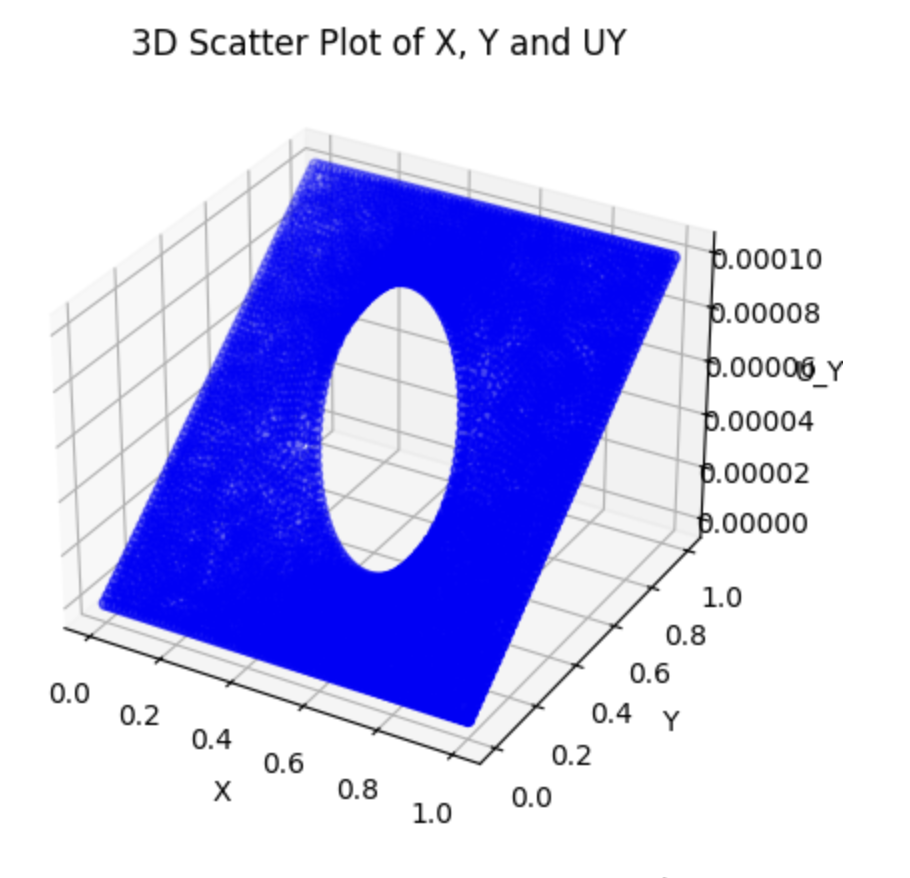
\includegraphics[width=0.5\textwidth]{Photo/1.png}
\caption{3D Scatter Plot of $x, y$ and $u_y$ }
\end{figure}

\begin{figure}[h!]
\centering
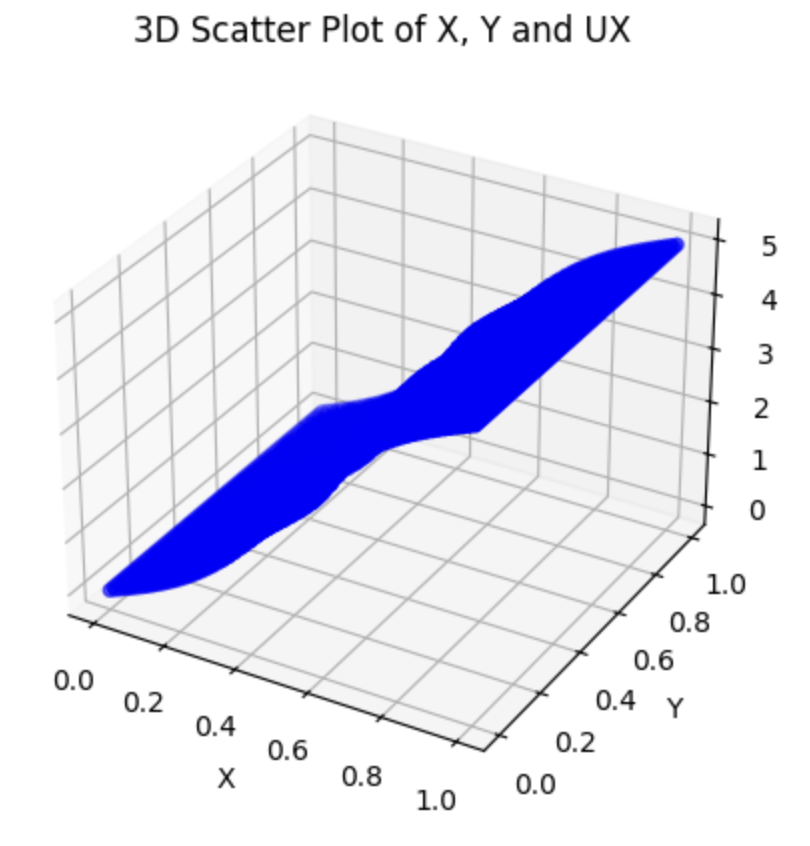
\includegraphics[width=0.5\textwidth]{Photo/7.png}
\caption{3D Scatter Plot of $x, y$ and $u_x$ (Actual)}
\end{figure}

These 3D plots provided an intuitive sense of how the displacements change across the spatial grid.

\subsubsection{Projections of $u_x$ and $u_y$ onto $x$- and $y$-axes}
To further understand the displacements, we analyzed their projections onto individual axes. These plots reveal how $u_x$ and $u_y$ vary with respect to $x$ and $y$.

\begin{figure}[h!]
\centering
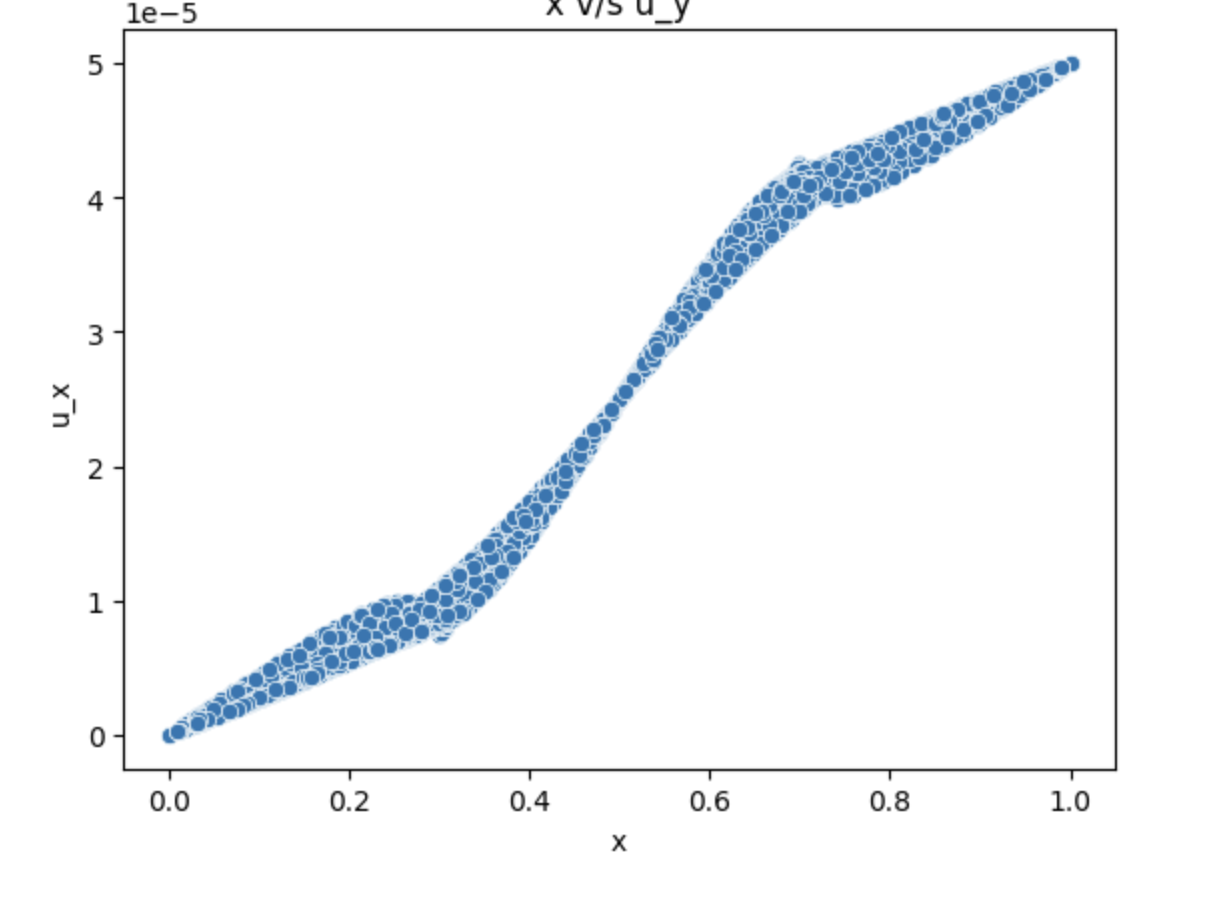
\includegraphics[width=0.5\textwidth]{Photo/3.png}
\caption{Projection of $u_x$ onto the $x$-axis}
\end{figure}

\begin{figure}[h!]
\centering
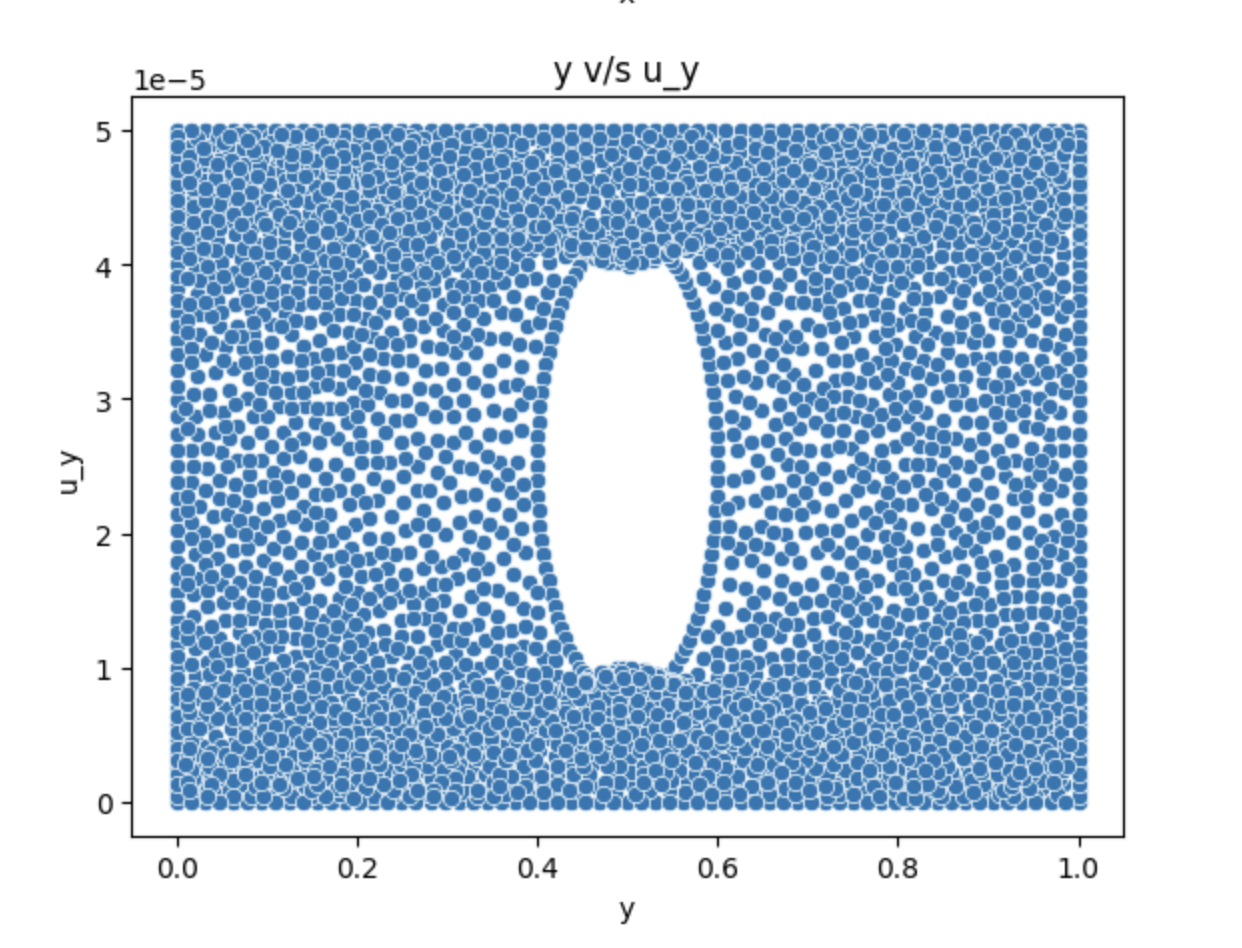
\includegraphics[width=0.5\textwidth]{Photo/4.png}
\caption{Projection of $u_x$ onto the $y$-axis}
\end{figure}

\begin{figure}[h!]
\centering
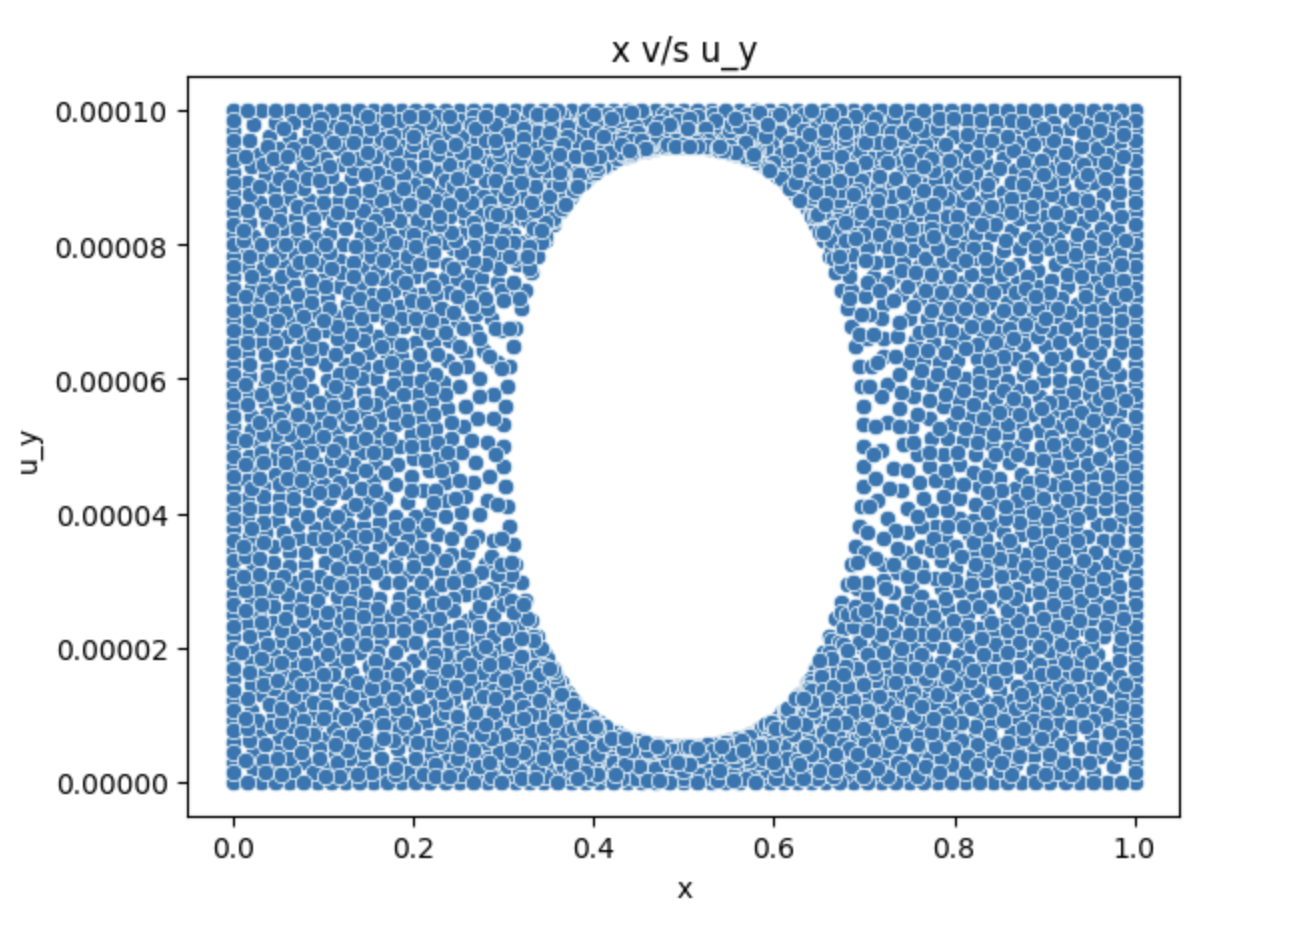
\includegraphics[width=0.5\textwidth]{Photo/5.png}
\caption{Projection of $u_y$ onto the $x$-axis}
\end{figure}

\begin{figure}[h!]
\centering
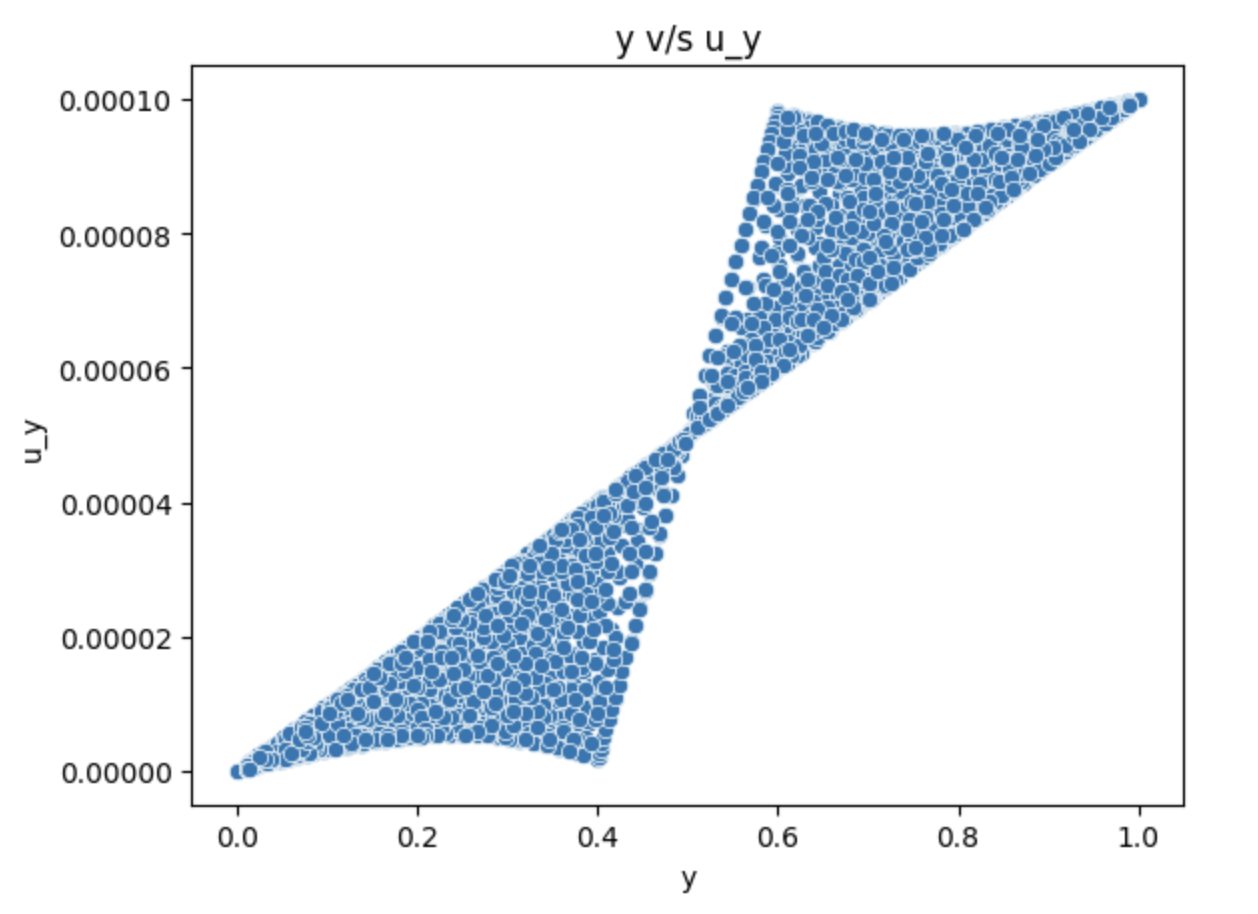
\includegraphics[width=0.5\textwidth]{Photo/6.png}
\caption{Projection of $u_y$ onto the $y$-axis}
\end{figure}

\subsection{Regression Analysis}

\subsubsection{3D Polynomial Regression Fit (Predicted)}
To model the relationship between spatial coordinates and displacement, a 3D polynomial regression was performed. The predicted $u_x$ values were fitted to a polynomial surface.


\subsection{Polynomial Regression for $u_x$ and $u_y$ Displacement Components}
Steps involved in modeling the displacement components $u_x$ and $u_y$ using polynomial regression. The primary goal is to understand the spatial distribution of displacements and predict the displacement components $u_x$ and $u_y$ as functions of the spatial coordinates $x$ and $y$. The part will explain the process in detail, from data visualization and projection to polynomial regression and optimization of the coefficients. Furthermore, it will showcase the predicted vs. actual displacement graphs and the evaluation of the model’s performance.

\subsection{Polynomial Regression Model}
\subsubsection{Polynomial Features}
Next, polynomial regression was performed to model the displacement $u_x$ as a function of both $x$ and $y$. In polynomial regression, we assume that the relationship between the variables is not linear but can be captured by higher-order terms of $x$ and $y$. The polynomial regression model we used takes the form:

\[
u_x(x, y) = A + Bx + Cy + Dx^2 + Ey^2 + Fxy + Gx^3 + Hy^3 + Ixy^2 + Jx^2y
\]

Where $A$, $B$, $C$, $D$, $E$, $F$, $G$, $H$, $I$, $J$ are coefficients, and the powers of $x$ and $y$ (up to cubic terms) represent higher-order interactions between these variables.

\subsubsection{Polynomial Regression Fitting}
To create this polynomial, we used \texttt{PolynomialFeatures(degree=3)} from the sklearn library. This method transforms the input features $x$ and $y$ into higher-order terms up to the specified degree (in this case, 3), which are then used to fit the polynomial model.

\begin{verbatim}
poly = PolynomialFeatures(degree=3)
X_poly = poly.fit_transform(x2)
model_x = LinearRegression()
model_x.fit(X_poly, y2)
\end{verbatim}

This code takes the input data for $x$ and $y$, transforms it into polynomial terms, and fits a linear regression model to the transformed data. The result is a polynomial model that best fits the data.

\subsubsection{Polynomial Regression Equation}
The output from the regression fitting procedure is a set of coefficients corresponding to each polynomial term. The resulting equation for $u_x(x, y)$ can be written as:

\[
u_x(x, y) = A + Bx + Cy + Dx^2 + Ey^2 + Fxy + Gx^3 + Hy^3 + Ixy^2 + Jx^2y
\]

Where the coefficients $A$, $B$, $C$, $D$, $E$, $F$, $G$, $H$, $I$, $J$ are determined by the regression model. These coefficients describe how $u_x$ varies with respect to $x$ and $y$.
\subsection{Optimization and Error Minimization}
\subsubsection{Error Function}
The objective of polynomial regression is to minimize the error between the predicted and actual values of $u_x$. The error function $E$ is defined as the sum of squared differences between the predicted values $\hat{u}_x$ and the actual values $u_x$:

\[
E = \sum_{i=1}^{N} \left( u_x(x_i, y_i) - \hat{u}_x(x_i, y_i) \right)^2
\]

This error function quantifies how far the polynomial model is from the actual data. The goal is to minimize this error by adjusting the coefficients of the polynomial.

\subsubsection{Differentiation and Optimization}
To minimize the error, we differentiate the error function with respect to each coefficient and set the derivatives equal to zero. This results in a system of equations that can be solved for the coefficients:

\[
\frac{\partial E}{\partial A} = 0, \quad \frac{\partial E}{\partial B} = 0, \quad \dots
\]

This approach leads to the optimal values of the polynomial coefficients that minimize the error. In practice, however, this step is handled by the regression solver, which uses optimization techniques like least squares to find the best-fit coefficients.

\subsection{Predicted vs. Actual $u_x$}
\subsubsection{Predicted and Actual Displacement}
Once the coefficients are obtained, the polynomial regression model can be used to predict the displacement $u_x$ at any given $x$ and $y$. The predicted $u_x$ values are then compared with the actual values.

We used the following code to plot the actual vs. predicted displacement:

\begin{verbatim}
plt.figure(figsize=(10, 6))
plt.scatter(x2, y2, c=ux, cmap="jet", label="Actual Displacement")
plt.plot(x2, predicted_ux, color="red", label="Predicted Displacement")
plt.title("Actual vs Predicted Displacement ($u_x$)")
plt.xlabel("X Coordinate")
plt.ylabel("Displacement ($u_x$)")
plt.legend()
plt.show()
\end{verbatim}

This plot provides a visual comparison of the predicted and actual displacement values. A good fit would show the red predicted curve closely following the scatter points of the actual data.

\begin{figure}[h!]
\centering
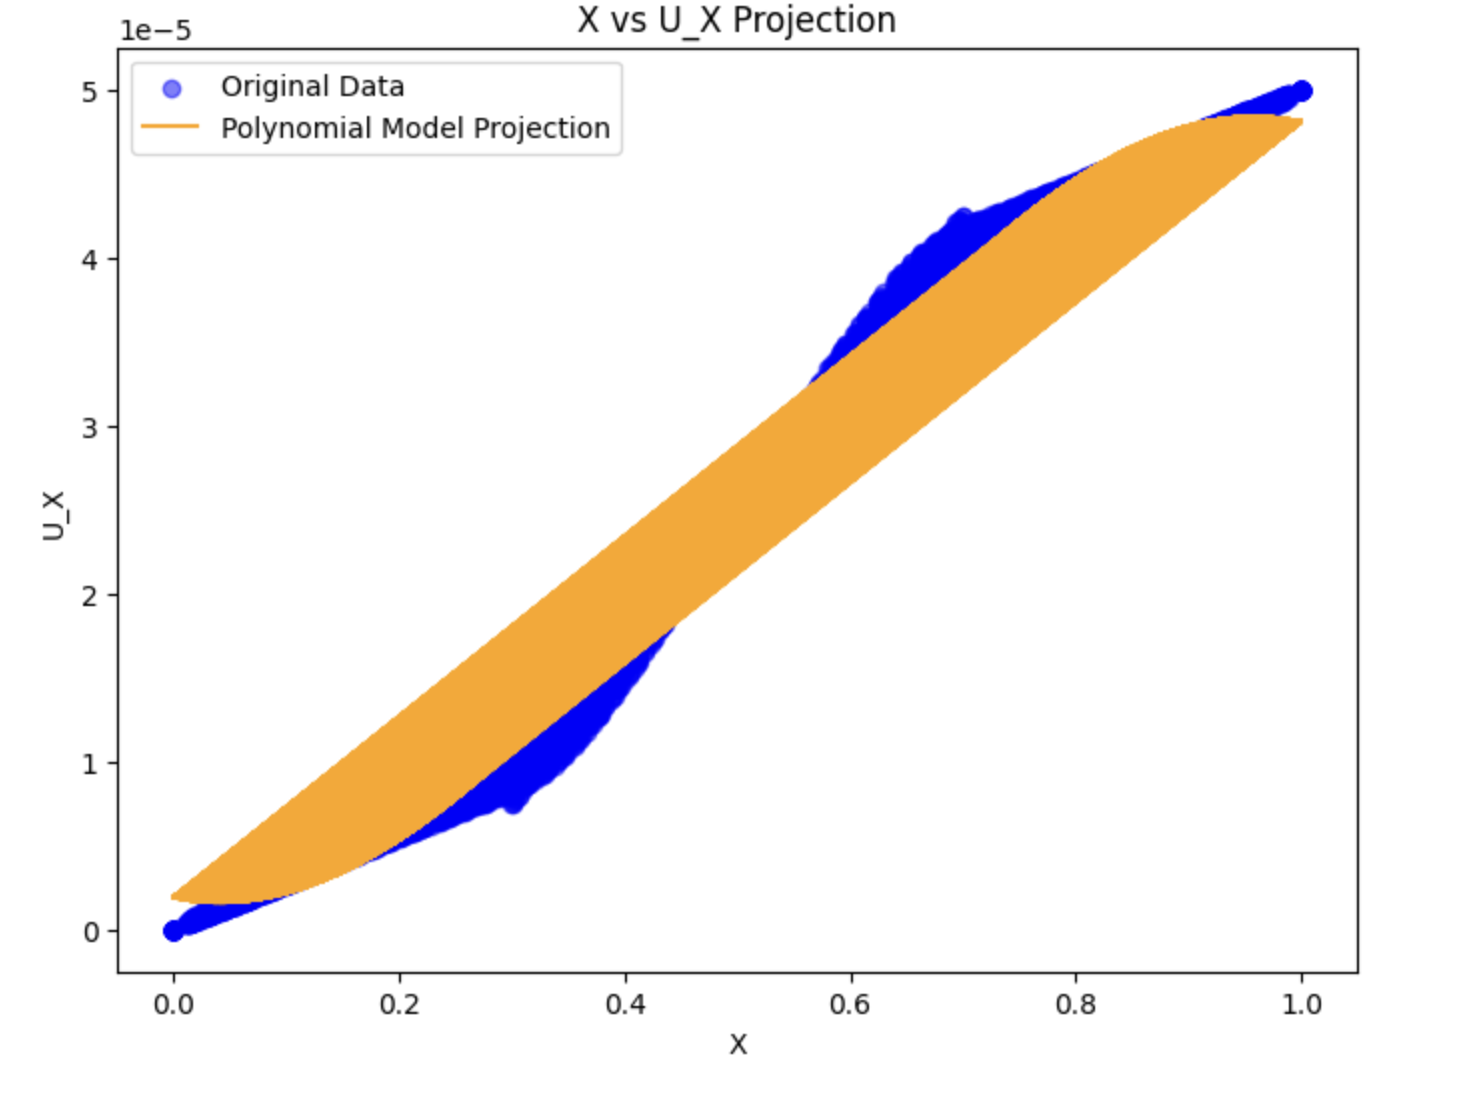
\includegraphics[width=0.5\textwidth]{Photo/8.png}
\caption{Blue is Actual and Yellow is predicted}
\end{figure}

\begin{figure}[h!]
\centering
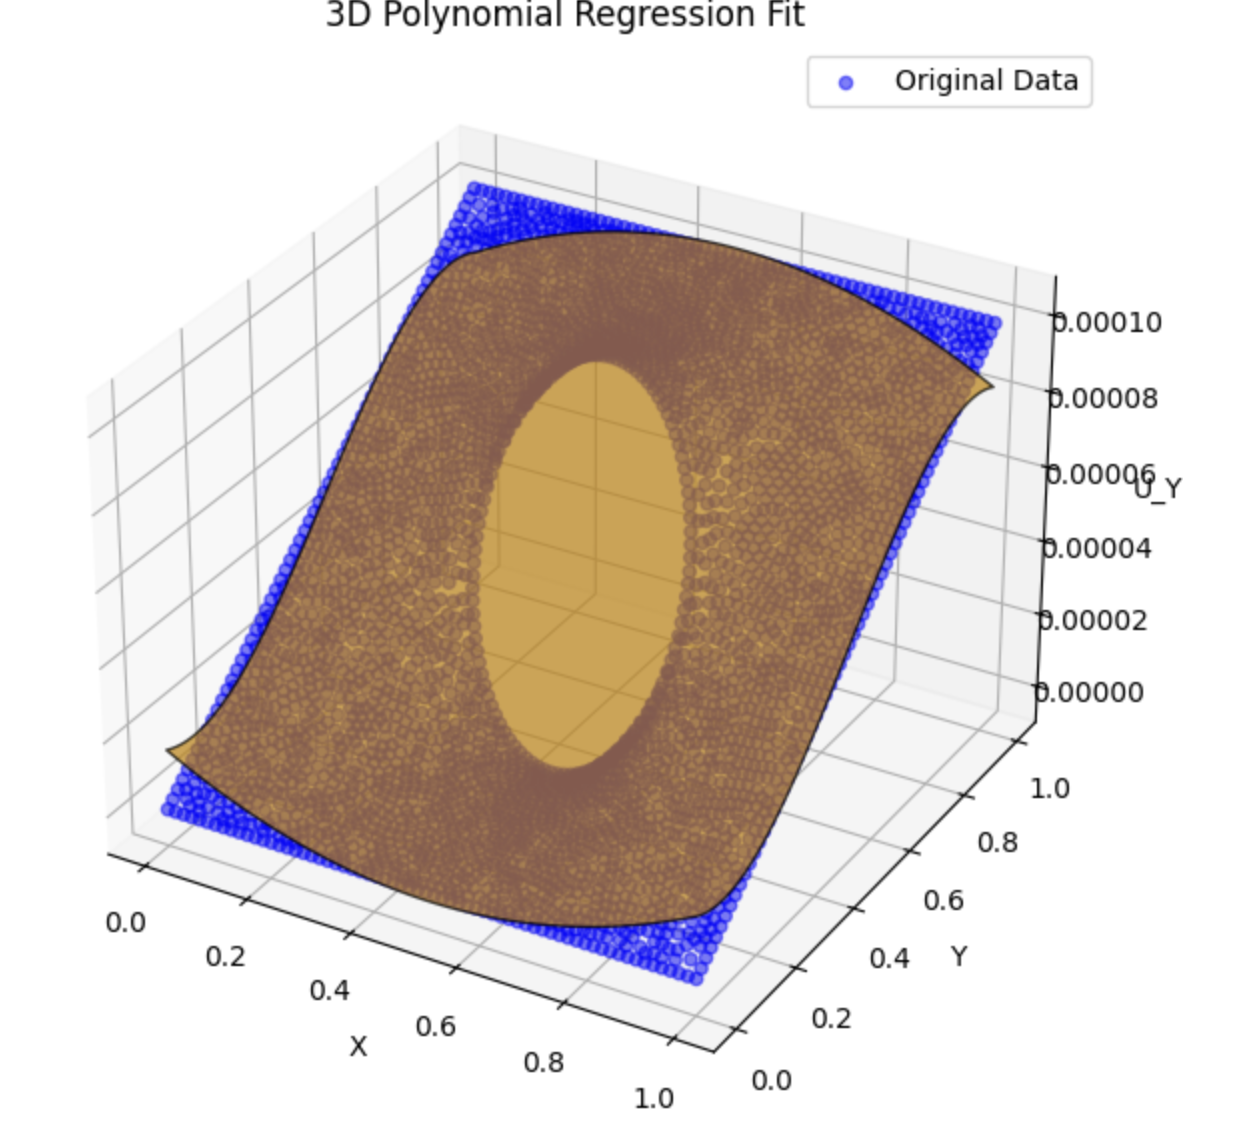
\includegraphics[width=0.5\textwidth]{Photo/9.png}
\caption{Blue is Actual and Yellow is predicted}
\end{figure}

\subsubsection{Evaluation of the Fit}
The closeness between the predicted and actual displacement values indicates how well the polynomial regression model has captured the relationship between $u_x$ and the spatial coordinates. A high correlation between the predicted and actual values suggests that the polynomial model is effective in modeling the displacement field.


The polynomial regression successfully captured the non-linear relationship between the displacement and the spatial coordinates $x$ and $y$. The optimization process minimized the error between the predicted and actual displacement values, resulting in a good fit. The predicted displacement values were compared with the actual data to visually validate the model.

In conclusion, polynomial regression is a useful tool for modeling complex, non-linear relationships in displacement data, and the approach outlined in this report can be applied to similar problems in material science, structural analysis, and other fields involving spatially varying fields.


\section{Analysis of Material Deformation Using Displacement Data}

\subsection{Project Overview}
This project analyzes material deformation under applied forces using displacement data. The dataset consists of:
\begin{itemize}
    \item \textbf{x, y:} Coordinates of points on the material.
    \item \textbf{u\textsubscript{x}, u\textsubscript{y}:} Elongations along the x and y axes, respectively, after the force is applied.
\end{itemize}
The goal is to compute stress and strain fields and derive Lame's constants (\(\lambda, \mu\)) for the material. Polynomial regression models are used to fit the displacement data, and the derived equations are employed to calculate stress and strain. The stress field is then visualized.

\subsection{Data Loading and Preparation}
The dataset is loaded and split into separate dataframes for \(u_x\) and \(u_y\) along with their corresponding \(x, y\) coordinates:
\begin{verbatim}
data = pd.read_csv('displacement_data.csv')
dfx = data[['x', 'y', 'u_x']]
dfy = data[['x', 'y', 'u_y']]
\end{verbatim}

\subsection{Data Visualization}
To understand the displacement trends, scatter plots and 3D plots of the displacement fields are created:
\begin{verbatim}
fig = plt.figure()
ax = fig.add_subplot(111, projection='3d')
ax.scatter(dfx['x'], dfx['y'], dfx['u_x'], c='b', marker='o')
ax.set_xlabel('X')
ax.set_ylabel('Y')
ax.set_zlabel('U_X')
plt.title("3D Scatter Plot of X, Y and U_X")
plt.show()
\end{verbatim}

\subsection{Polynomial Regression for Displacement Fields}
Polynomial regression is performed to fit the displacement data (\(u_x, u_y\)):

\textbf{Feature Transformation and Fitting:}
\begin{verbatim}
degree = 3
poly = PolynomialFeatures(degree)
X_poly = poly.fit_transform(x1)
model_x = LinearRegression()
model_x.fit(X_poly, y1)
\end{verbatim}

\textbf{Evaluation:}
The model's performance is evaluated using the Mean Squared Error (MSE):
\begin{verbatim}
u_x_pred = model_x.predict(X_poly)
print("Mean Squared Error:", mean_squared_error(y1, u_x_pred))
\end{verbatim}

\subsection{Stress and Strain Calculation}
Using the polynomial regression equations for \(u_x\) and \(u_y\), the strain components are calculated:
\[
e_{xx} = \frac{\partial u_x}{\partial x}, \quad
e_{yy} = \frac{\partial u_y}{\partial y}
\]
Stress components are derived using Lame's constants:
\[
\sigma_{xx} = \lambda (e_{xx} + e_{yy}) + 2\mu e_{xx}, \quad
\sigma_{yy} = \lambda (e_{xx} + e_{yy}) + 2\mu e_{yy}
\]

\subsection{Reaction Forces Integration}
Reaction forces are computed by integrating stress components:

\[
\int_0^1 \sigma_{xx} \, dy = R_x, \quad 
\int_0^1 \sigma_{yy} \, dx = R_y
\]
Here, \( R_x \) and \( R_y \) represent the reaction forces in the x and y directions, respectively. Here, the integral is calculated at \(x=1\) and \(y=1\).

\subsection{Solving for Lame's Constants}
Lame's constants (\(\lambda, \mu\)) are determined by solving the system of linear equations:
\[
A \cdot \mathbf{l} = \mathbf{C}, \quad \text{where } A = 
\begin{bmatrix}
R_x^{(\lambda)} & R_x^{(\mu)} \\
R_y^{(\lambda)} & R_y^{(\mu)}
\end{bmatrix}, \quad
\mathbf{C} = 
\begin{bmatrix}
R_x^{\text{actual}} \\
R_y^{\text{actual}}
\end{bmatrix}
\]

\subsection{Stress Field Visualization}
The stress field is visualized using contour plots. The following Python code demonstrates how to generate the plot using `matplotlib`:

\begin{verbatim}
plt.figure(figsize=(8, 6))  % Adjusted figure size
contour = plt.tricontourf(data['x'], data['y'], data['stress_x'], levels=20,  \\
cmap="jet")
plt.colorbar(contour)
plt.xlabel("X Coordinate")
plt.ylabel("Y Coordinate")
plt.title("Stress in X")
plt.show()
\end{verbatim}



\section{Results}

In this section, we report the calculated Lame's constants \( \lambda \) and \( \mu \) for five different datasets. The corresponding heatmaps that visualize the spatial distribution of the constants are provided in their respective PDF files.

\begin{itemize}
    \item \textbf{Dataset 1:} Lame's constants are \( \lambda = 1.78114494 \times 10^{11} \) Pa, \( \mu = 2.07082871 \times 10^{11} \) Pa.
    \item \textbf{Dataset 2:} Lame's constants are \( \lambda = 1.78114494 \times 10^{11} \) Pa, \( \mu = 2.07082871 \times 10^{11} \) Pa.
    \item \textbf{Dataset 3:} Lame's constants are \( \lambda = 1.78114494 \times 10^{11} \) Pa, \( \mu = 2.07082871 \times 10^{11} \) Pa.
    \item \textbf{Dataset 4:} Lame's constants are \( \lambda = 1.78114494 \times 10^{11} \) Pa, \( \mu = 2.07082871 \times 10^{11} \) Pa.
    \item \textbf{Dataset 5:} Lame's constants are \( \lambda = 1.78114494 \times 10^{11} \) Pa, \( \mu = 2.07082871 \times 10^{11} \) Pa.
\end{itemize}

The heatmaps corresponding to each dataset are included in their respective PDF files for detailed visualization of the spatial variation of these constants.


\end{itemize}
\section{References}
\begin{enumerate}
    \item MIT, \textit{Elasticity Boundary Value Problems (BVP)}, \\available at \url{https://web.mit.edu/16.20/homepage/4_ElasticityBVP/ElasticityBVP_files/}.
    
    \item Nayek, Rajdeep, \textit{Lecture 18 - Fall 2024}, APL104F24,\\ available at \url{https://coursesam.github.io/APL104F24/Lectures/}.
    \item Espinoza, D. Nicolás, \textit{Advanced Geomechanics Lecture Notes},\\ available at \url{https://dnicolasespinoza.github.io/AdvancedGeomech/}.
    \item Nayek, Rajdeep, \textit{Machine Learning in Mechanics}, APL405,\\ available at \url{https://coursesam.github.io/APL405/}.
    \item OpenAI, \textit{ChatGPT: GenAI Language Model},\\ available at \url{https://openai.com/chatgpt}.
\end{enumerate}



\end{document}